\documentclass{book}

\usepackage{listings}
\usepackage{theorem}
\usepackage{graphicx}
\usepackage{hyperref}
\usepackage{amsfonts}
\usepackage{amsmath}
\usepackage[table]{xcolor}
\usepackage{array,calc}
\usepackage{amsmath}

\newtheorem{exercise}{Exercise}


\lstset{
  language=Java,
  basicstyle=\ttfamily\footnotesize,
  numbers = left
}

\newcommand{\co}[1]{\lstinline[language=Java, basicstyle=\ttfamily]{#1}}

\begin{document}

\addtocounter{chapter}{2}

\chapter{Image Histograms}

\section{Grayscale Image Histograms}
An image histogram describes how frequently each color occurs within an image. For example, consider the grayscale image and the corresponding histogram shown below.
\begin{center}
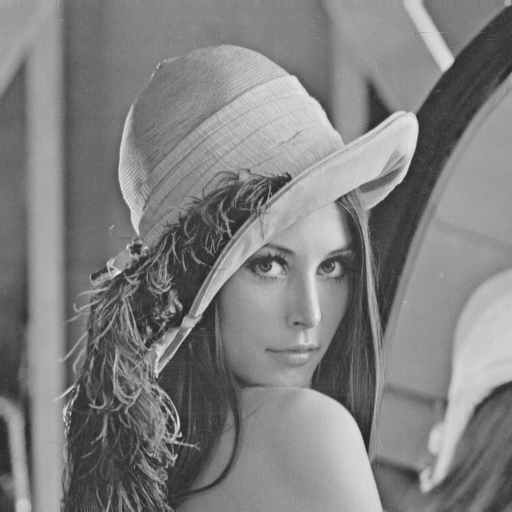
\includegraphics[scale=0.15]{lena-gray.png}
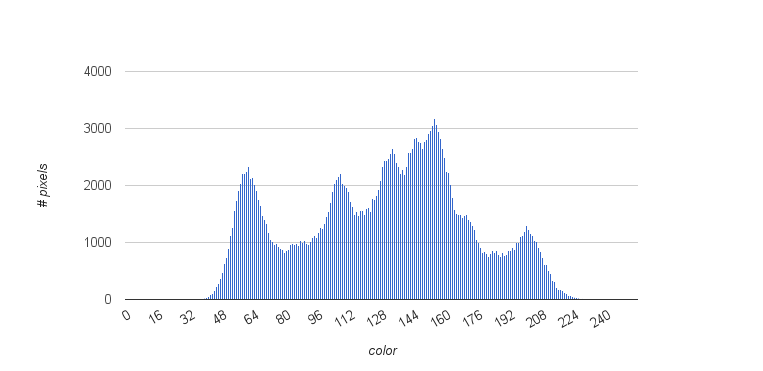
\includegraphics[scale=0.5]{lena-gray-histogram.png}
\end{center}
The X-axes of the histogram contains the values 0 to 255, representing colors in the 8-bit grayscale image. The Y-axes displays the number of pixels per color. For example, \texttt{lena-gray.png} contains 0 black pixels, 1463 pixels with value 100, 2804 pixels with value 150, etc.

\begin{exercise}
Is it possible to reconstruct an image from an histogram?
\end{exercise}

More formally, an image histogram $h$ is a function that maps each color $c$ to the number of pixels with that color in the image $I$:
$$h(c) = |\{ (x, y) \mid I(x, y) = c \}|$$
for each color $c$.

\begin{exercise}\label{ex:histogram}
Write a class \co{Gray8Histogram} to compute histograms for grayscale images.
\begin{itemize}
  \item Add a field named \co{histogram} with type \co{int[]} to the class \co{Gray8Histogram}. Initialize this field to an integer array of length 256. The goal of this field is to store the number of pixels of each color. For example, \co{histogram[20]} will contain the number of pixels with color \co{20}.
  \item Add a constructor with a parameter of type \co{ImageProcessor}. The constructor should compute the histogram for the given image.
  \item Add a method \co{getNbPixelsWithColor} that returns the number of pixels with the given color in constant time.
  \item Add a method \co{print} that prints the histogram to standard out. The output of this method should look as follows:
\begin{verbatim}
#pixels with color 0: 10
#pixels with color 1: 43
#pixels with color 2: 0
...
\end{verbatim}
 \item Add a method \co{display} that visualizes the histogram in a new window as a graph. Use the class \href{http://rsbweb.nih.gov/ij/developer/api/ij/gui/Plot.html}{\texttt{ij.gui.Plot}} to do so. In particular, the body of \co{display} should create a new \co{Plot} and call \co{show} to display this \co{Plot} in a new window as follows: 
 \begin{lstlisting}
 Plot plot = new Plot("histogram", "color", "# pixels",
   xValues, yValues);
 plot.show();
 \end{lstlisting}
Here, \co{xValues} and \co{Y-values} contain the data displayed on the X and Y-axes graph. Both arrays should have length 256. \co{xValues} should contain the values 0 to 255, while Y-array should contain the values in the field \co{histogram}.
\end{itemize} 
\end{exercise}

\begin{exercise}
Display the histogram of the image located at

 \href{http://www.cs.kuleuven.be/~jans/histogramquestion.png}{http://www.cs.kuleuven.be/~jans/histogramquestion.png} 
 
by reading it via a \co{URL}. Do not look at the image yet. What can you say about the image based on the histogram? Check your predictions. 
\end{exercise}

We define the \emph{dynamic range} of an image as the number of distinct pixel values in that image. Similarly, the \emph{contrast} of an image is the difference between the minimum and maximum pixel value in that image. For example, the minimum and maximum pixel values in \co{lena-gray.png} are respectively $35$ and $240$, and hence the contrast of the image is $205$.

\begin{exercise}
Extend the class \co{Gray8Histogram} with four additional methods: \co{getMin}, \co{getMax}, \co{getContrast} and \co{getDynamicRange}. \co{getMin} and \co{getMax} respectively the minimum and maximum pixel value occurring in the image. 
\end{exercise}

\section{Cumulative Grayscale Image Histograms}
A histogram describes fore each color the number of pixels with exactly that color. A cumulative histogram on the other hand describes for each color the number of pixels with a value less than or equal to that color. The cumulative histogram for \texttt{lena-gray.png} is shown below:
\begin{center}
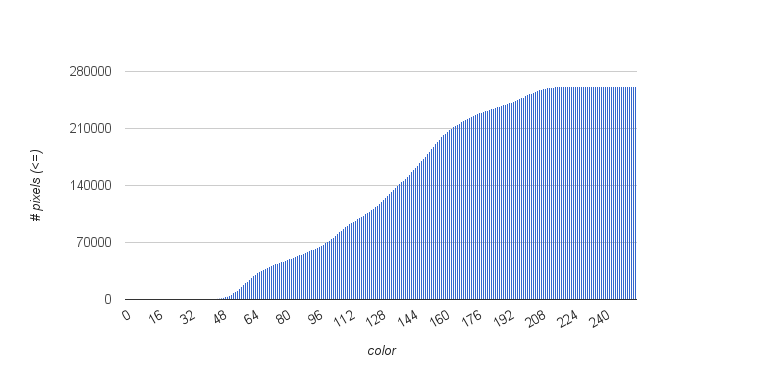
\includegraphics[scale=0.5]{lena-gray-cumulative-histogram.png}
\end{center}
For example, the number of pixels with value less than or equal to 100 is 69533.

More formally, a cumulative image histogram $H$ is a function that maps each color $c$ to the number of pixels with value less or equal to $c$ in the image $I$:
$$H(c) = |\{ (x, y) \mid I(x, y) \leq c \}|$$
for each color $c$. Alternatively, we can recursively define the cumulative histogram $H$ based on the normal histogram $h$ as follows:
$$H(c) = \left\{\begin{array}{c l}
  h(0) & \text{if $c = 0$}\\
  h(c) + H(c - 1) & \text{if $0 < c \leq 255$}\\
\end{array}
\right.$$
for each color $c$.

\begin{exercise}
Write a new class \co{Gray8CumulativeHistogram}.
\begin{itemize}
  \item  Add a field named \co{cumulativeHistogram} with type \co{int[]} to the class \co{Gray8CumulativeHistogram}. Initialize this field to an integer array of length 256. The goal of this field is to store the number of pixels with value less than or equal to a given color. For example, \co{cumulativeHistogram[20]} will contain the number of pixels with value less than or equal to \co{20}.
  \item Add a constructor with a parameter of type \co{Gray8Histogram}. The constructor should compute the cumulative histogram for the given image based on the normal histogram.
   \item Add a method \co{getNbPixelsWithColorLessThanOrEqualTo} that returns the number of pixels with value less than or equal to the given color in constant time.
  \item Add a method \co{print} that prints the cumulative histogram to standard out. 
 \item Add a method \co{display} that visualizes the cumulative histogram in a new window as a graph.
\end{itemize}
\end{exercise}

\begin{exercise}
What is the value corresponding to color 255 in each cumulative histogram?  
\end{exercise}

\section{Color Image Histograms}
What does the term `histogram' refer to in the context of color images?

\subsection{Individual Color Channel Histogram}
Each pixel in an RGB color image consists of three separate channels: red, green and blue. An RGB color image can therefore be decomposed into three grayscale images, one for each channel. For example, the three grayscale corresponding to \co{lena.png} are shown below.
\begin{center}
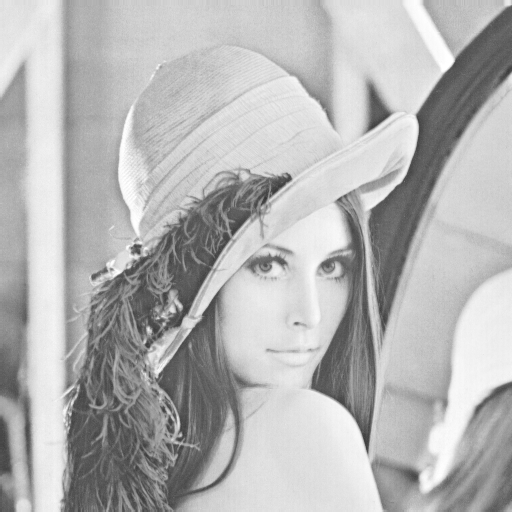
\includegraphics[scale=0.2]{lena-red.png}
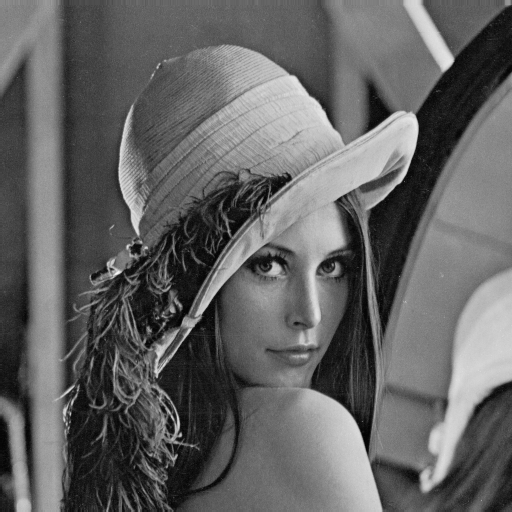
\includegraphics[scale=0.2]{lena-green.png}
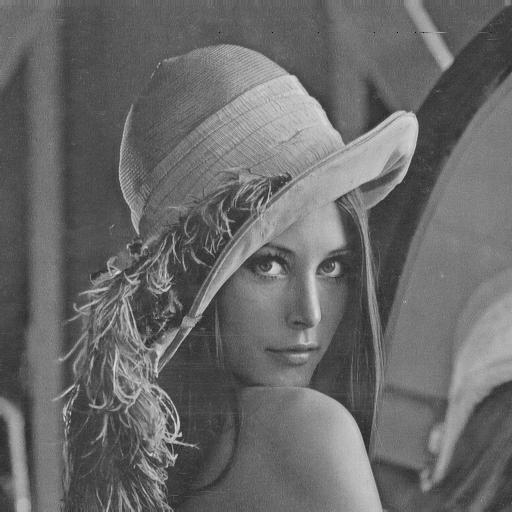
\includegraphics[scale=0.2]{lena-blue.png}
\end{center}
The histograms of the individual color channels are often used as the histogram of the RGB color image. These individual histograms are typically shown in the same plot in different colors as shown below:
\begin{center}
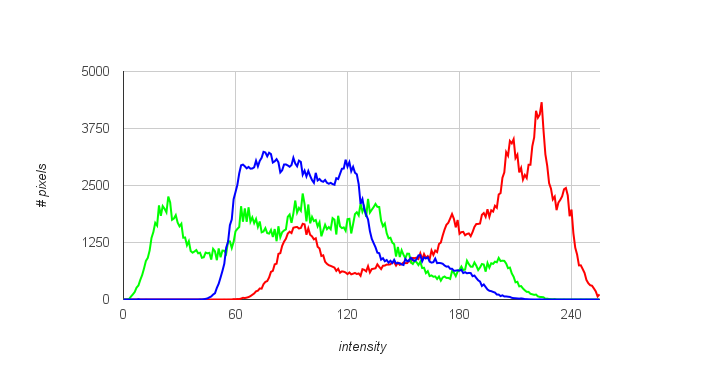
\includegraphics[scale=0.5]{lena-histogram.png}
\end{center}

\begin{exercise}
Write a new class \co{RGBHistogram}.
\begin{itemize}
  \item  Add fields named \co{redHistogram}, \co{greenHistogram} and \co{blueHistogram} with type \co{Gray8Histogram} to the class \co{RGBHistogram}.
  \item Add a constructor with a parameter named \co{cp} of type \co{ColorProcessor}. \co{ColorProcessor} is a subtype of \co{ImageProcessor} used for processing RGB color images. The method \co{ColorProcessor.getChannel} can be used to retrieve the bytes corresponding to each individual color channel. For example, \co{cp.getChannel(1)} returns a byte array representing the red channel.
  
 The constructor should initialize the histograms for the three color channels of the given image as follows:
  \begin{lstlisting}
int w = cp.getWidth();
int h = cp.getHeight();
redHistogram = new Gray8Histogram(
  new ByteProcessor(w, h, cp.getChannel(1), null));
greenHistogram = new Gray8Histogram(
  new ByteProcessor(w, h, cp.getChannel(2), null));
blueHistogram = ...
  \end{lstlisting}
   \item Add a method \co{getNbPixelsWithRedChannel} that returns the number of pixels where the red component equals the given value in constant time. Add similar methods for green and blue.
  \item Add a method \co{print} that prints the histogram to standard out. The output of this method should look as follows:
\begin{verbatim}
#pixels with intensity 0: red=0, green=24, blue=0  
#pixels with intensity 1: red=5, green=4, blue=54 
...
\end{verbatim}
 \item Add a method \co{display} that visualizes the histogram of the three channels in a new window as a graph. Pass the data for the red channel via the constructor and use \co{Plot.addPoints} to add the data for the other two channels. The color of the plotted lines can be modified via \co{setColor}. 
\end{itemize}
\end{exercise}

\subsection{Luminance Histogram}
The luminance histogram of a color image is the histogram of the corresponding luminance image. That is, each pixel in an RGB color image has a luminance. The luminance $Y$ of an RGB triple (R, G, B) is a weighted sum of the the individual channels:
$$Y =  0.21 R + 0.72 G + 0.07 B$$
These weights reflect the fact that the human eye is more sensitive to green light than to blue light. The luminance of each pixel is value between 0 and 255, and hence the luminance image is a grayscale image.
\end{document}
